% small.tex
\documentclass[t]{beamer}
\usepackage{graphicx}
\usepackage{listliketab}
\usepackage[absolute,overlay]{textpos}
\usetheme[hideothersubsections]{Goettingen}
\setbeamercolor{palette primary}{bg=structure.fg!25}
\setbeamercolor{palette secondary}{bg=structure.fg!10,fg=black}
\useinnertheme{rectangles} 
\useoutertheme{infolines} 
\author[T.A.E.Smith]{Thomas Smith} 
\title[CM50175]{CM50175\\Research Project Preparation}
\institute[Bath/CS]{Centre for Digital Entertainment\\University of Bath}
\date{April 20, 2014} 
\begin{document}

% Just to remind people that the final presentations should be about your entire project, focussing on the problem, your anticipated solution and the key references from the relevant literature.

%--- the titlepage frame -------------------------%
\begin{frame}
	\titlepage
\end{frame}

%--- the presentation begins here ----------------%
\section{Context}
	\subsection{Born Ready Games}
		\begin{frame}{Born Ready Games}
			\begin{textblock*}{2cm}[0,1](.5cm,8.9cm) % {block width} (coords)
			
\includegraphics[width=2cm]{bornready.jpg}
			\end{textblock*}
			\begin{textblock*}{2cm}[0,1](8.3cm,8.9cm) % {block width} (coords)
			
\includegraphics[width=2cm]{strikesuitzero.jpg}
			\end{textblock*}
			\begin{itemize}
				\item Guildford-based `indie' games studio
				\item Sucessful `Strike Suit' franchise
				\begin{itemize}
					\item Two games across five platforms
					\item Space-based fighter combat at large scale
					\item `Play a key role in a larger story'
				\end{itemize}
				\item In-house art team, publishing, PR
			\end{itemize}
			\begin{center}
				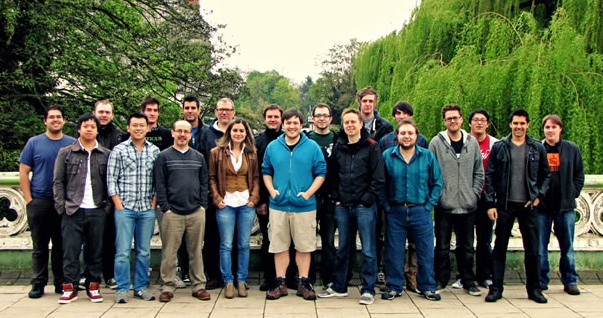
\includegraphics[width=0.5\linewidth]{team.jpg}
			\end{center}
		\end{frame}

		\begin{frame}{Born Ready Games --- Strike Suit Zero}
			\begin{textblock*}{2cm}[0,1](.5cm,8.9cm) % {block width} (coords)
			
\includegraphics[width=2cm]{bornready.jpg}
			\end{textblock*}
			\begin{textblock*}{2cm}[0,1](8.3cm,8.9cm) % {block width} (coords)
			
\includegraphics[width=2cm]{strikesuitzero.jpg}
			\end{textblock*}
			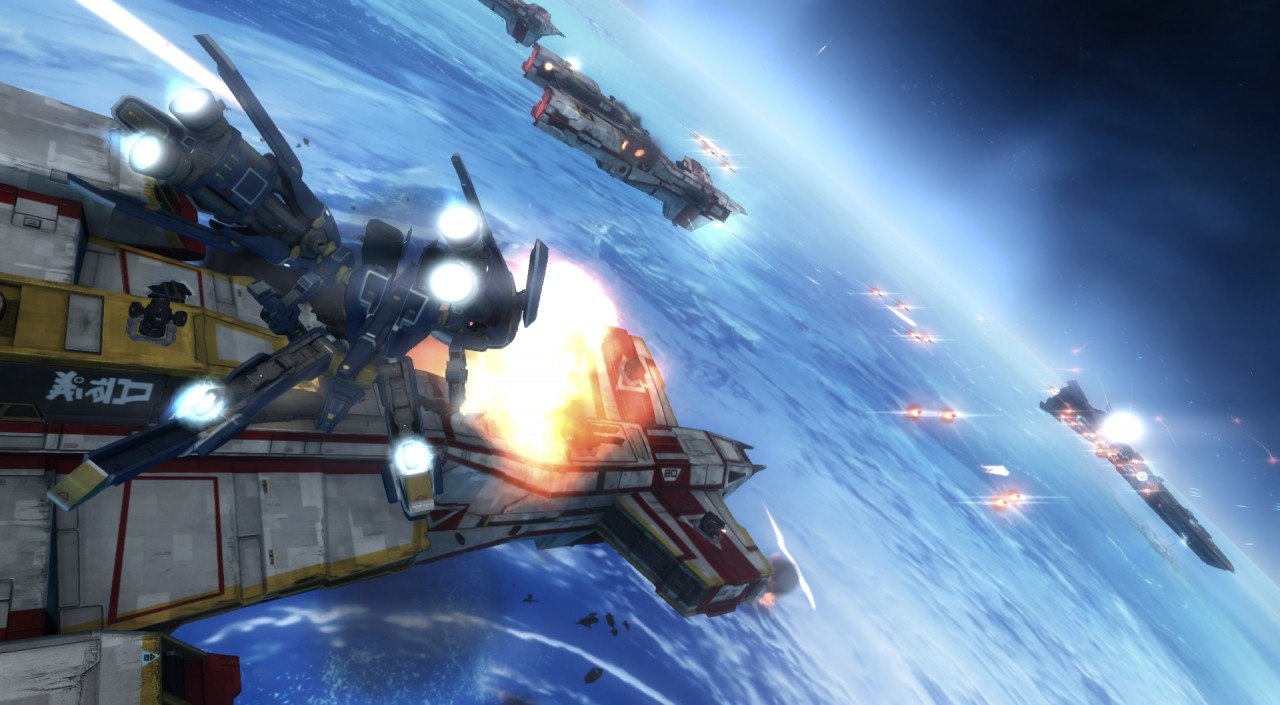
\includegraphics[width=\linewidth]{capital.jpg}
			\begin{center}
				Strike Suit and capital ships
			\end{center}
		\end{frame}

		\begin{frame}{Born Ready Games --- Strike Suit Zero}
			\begin{textblock*}{2cm}[0,1](.5cm,8.9cm) % {block width} (coords)
			
\includegraphics[width=2cm]{bornready.jpg}
			\end{textblock*}
			\begin{textblock*}{2cm}[0,1](8.3cm,8.9cm) % {block width} (coords)
			
\includegraphics[width=2cm]{strikesuitzero.jpg}
			\end{textblock*}
			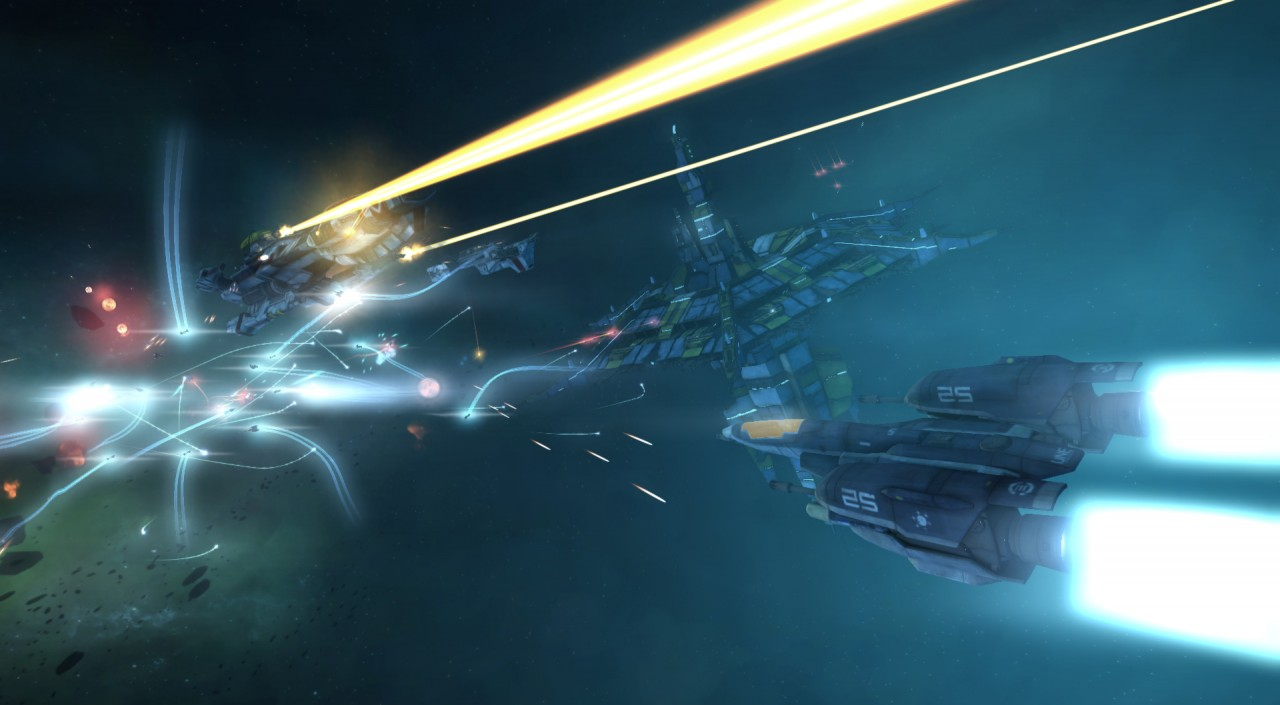
\includegraphics[width=\linewidth]{station.jpg}
			\begin{center}
			AXE fighter craft and \\
			Thule research station
			\end{center}
		\end{frame}

	\subsection{Art Pipeline}
		\begin{frame}{Art Pipeline}
			\begin{textblock*}{2cm}[0,1](.5cm,8.9cm) % {block width} (coords)
			
\includegraphics[width=2cm]{bornready.jpg}
			\end{textblock*}
			\begin{textblock*}{2cm}[0,1](8.3cm,8.9cm) % {block width} (coords)
			
\includegraphics[width=2cm]{strikesuitzero.jpg}
			\end{textblock*}
			\begin{itemize}
				\item High production overheads per asset
				\item Duplication of effort
				\begin{itemize}
					\item Pristine mesh and textures
					\item Damaged mesh and textures
					\item Destroyed mesh and textures
				\end{itemize}
				\item Static damage-based system for swapping meshes
				\item Procedural impulse vectors for detroyed meshes
				\item Larger ships have independent weapon hardpoints
				\item Relatively low variety of ship models in current game
			\end{itemize}
		
		\end{frame}


	\subsection{Procedural Destruction}
		\begin{frame}{Procedural Destruction}
		\begin{quote} \footnotesize
		``The aim of the project is to explore and implement a declarative approach to the modelling of structure, so that reasoning about the effects of damage can take place over a knowledge-based representation from which a rendering can be synthesized automatically.  The representation evolves over time in response to the damage inflicted, but could also be subject to other forms of failure arising from other environmental events.''
		\end{quote}
		\hfill --- J. A. Padget
		\end{frame}

		\begin{frame}[noframenumbering]{Procedural Destruction}
		\begin{quote} \footnotesize
		``The aim of the project is to explore and implement a declarative approach to the modelling of structure, so that reasoning about the effects of damage can take place over a knowledge-based representation from which a rendering can be \textbf{synthesized automatically}.  The representation evolves over time in response to the damage inflicted, but could also be subject to other forms of failure arising from other environmental events.''\end{quote}
		\hfill --- J. A. Padget
		\begin{itemize}
			\item Research and build a procedural destruction system
			\item Generate custom damaged and destroyed appearances
				\begin{itemize}
					\item Structure-dependent deformation
					\item Realistic response to damage type
				\end{itemize}
			\item Real-time performance necessary
		\end{itemize}
		\end{frame}

		\begin{frame}{Context --- Sample Capital Ships}
			\begin{textblock*}{2cm}[0,1](.5cm,8.9cm) % {block width} (coords)
			
\includegraphics[width=2cm]{bornready.jpg}
			\end{textblock*}
			\begin{textblock*}{2cm}[0,1](8.3cm,8.9cm) % {block width} (coords)
			
\includegraphics[width=2cm]{strikesuitzero.jpg}
			\end{textblock*}
			\vskip 1em
			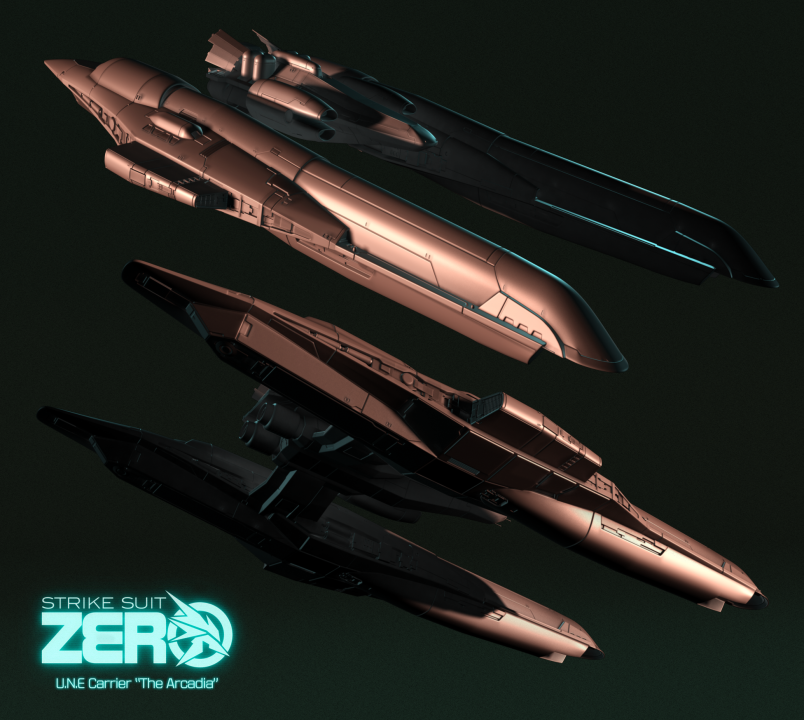
\includegraphics[width=0.46\linewidth]{arcadia.png}%
			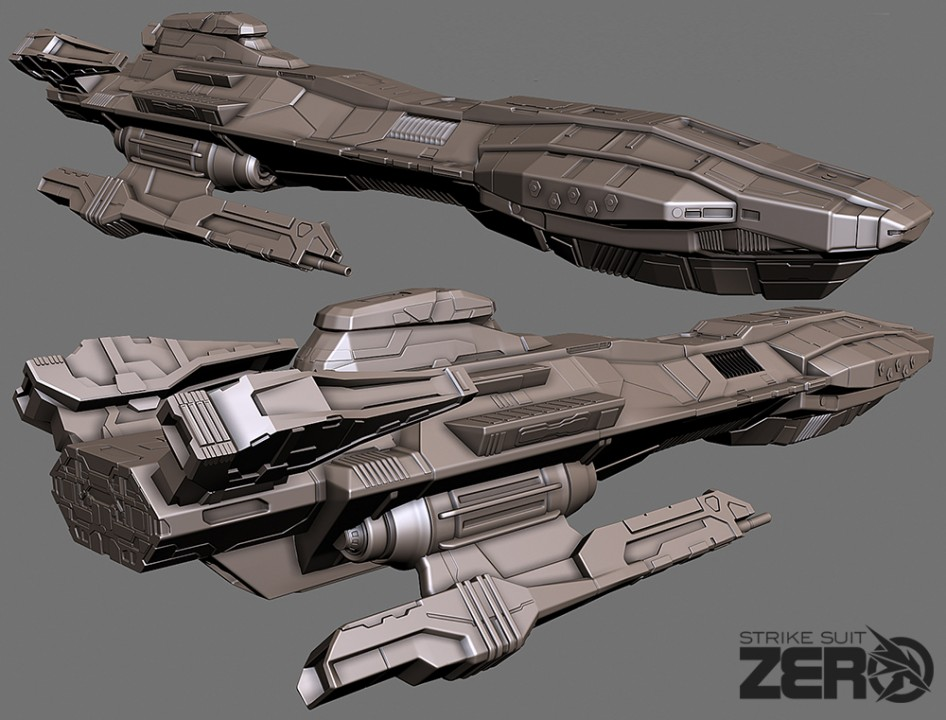
\includegraphics[width=0.54\linewidth]{muge2.jpg}\\
			U.N.E carrier `The Arcadia' \hfill MUGE-class cruiser
		\end{frame}
		\begin{frame}[c]{Context --- Size Comparison}
			\begin{textblock*}{2cm}[0,1](.5cm,8.9cm) % {block width} (coords)
			
\includegraphics[width=2cm]{bornready.jpg}
			\end{textblock*}
			\begin{textblock*}{2cm}[0,1](8.3cm,8.9cm) % {block width} (coords)
			
\includegraphics[width=2cm]{strikesuitzero.jpg}
			\end{textblock*}
			\vskip -1em
			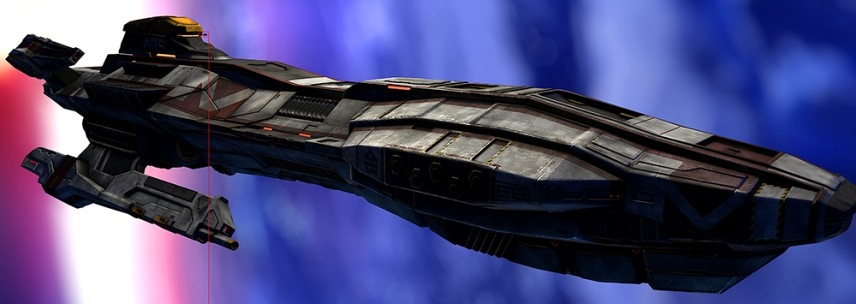
\includegraphics[width=\linewidth]{muge1.jpg}\begin{center}
			AXE fighter craft vs. MUGE-class cruiser
			\end{center}
		\end{frame}


\section{Existing Approaches}
	\begin{frame}{Existing Approaches}

	
	\end{frame}
	\subsection{Art Swap}
		\begin{frame}{Art Swap}
		\begin{itemize}
			\item Current implementation --- in-engine support
			\item Popular solution, used by many other games
			\item Low runtime cost --- damage thresholding
		\end{itemize}
		\emph{However:}
		\begin{itemize}
			\item High production cost - multiple asset versions
			\item Visually identical for every instance
		\end{itemize}
		
		\end{frame}
	\subsection{Material-based destruction}
		\begin{frame}{Material-based destruction}
		\end{frame}
	% \subsubsection{Havok Destruction}
	% \subsubsection{Euphoria}
	\subsection{Structure-aware solvers}
		\begin{frame}{Structure-aware solvers}
		\end{frame}


\section{Proposed Approach}
	\begin{frame}{Proposed Approach}
	\end{frame}
	\subsection{Answer Set Programming}
		\begin{frame}{Answer Set Programming}
		\end{frame}
	\subsection{Integrated Tools}
		\begin{frame}{Integrated Tools}
		\end{frame}

	\subsection{Benefits}
		\begin{frame}{Benefits}
		\end{frame}

\section{Conclusion}

% \section{}
% \begin{frame}{Glossary}
% \end{frame}

\end{document}